\documentclass[aspectratio=169,10pt]{beamer}
% build with   lualatex -shell-escape
% see makefile

% fallback search path for ../theme/ when TEXINPUTS is not set (e.g. texmaker
% quick build); the makefile's TEXINPUTS takes precedence, so no conflict
\makeatletter
\providecommand*{\input@path}{}
\edef\input@path{\input@path{../theme/}{../theme/moloch/}}
\makeatother

\usepackage{icl26}
\deftranslation[to=English]{Theorem}{theorem}
\deftranslation[to=English]{Definition}{definition}
\deftranslation[to=English]{Definitions}{definitions}
\deftranslation[to=English]{Lemma}{lemma}
\newtheorem{proposition}[theorem]{proposition}
\newtheorem{conjecture}[theorem]{conjecture}

\usepackage{multimedia}

\newcommand{\bg}{\mathbf{g}}
\newcommand{\bn}{\mathbf{n}}
\newcommand{\bq}{\mathbf{q}}
\newcommand{\bu}{\mathbf{u}}
\newcommand{\bv}{\mathbf{v}}

\newcommand{\bU}{\mathbf{U}}

\newcommand{\bzero}{\symbf{0}}

\newcommand{\cK}{{\mathcal{K}}}
\newcommand{\cQ}{{\mathcal{Q}}}
\newcommand{\cV}{{\mathcal{V}}}
\newcommand{\cX}{{\mathcal{X}}}

\newcommand{\RR}{{\mathbb{R}}}

\newcommand{\nn}{\mathrm{n}}
\newcommand{\pp}{\mathrm{p}}
\newcommand{\qq}{\mathrm{q}}
\newcommand{\rr}{\mathrm{r}}

\newcommand{\eps}{\epsilon}

\newcommand{\grad}{\nabla}
\newcommand{\Div}{\nabla\cdot}

\newcommand{\rhoi}{\rho_{\text{i}}}

\newcommand{\jump}[1]{[\![#1]\!]}

\newcommand{\lc}{{\text{\large $\circ$}}}

% grey comments on the right
\newcommand{\afcomm}[1]{\ensuremath{\text{\footnotesize \grey{$\leftarrow$ #1}}}}
\newcommand{\pcomm}[1]{\grey{\small (#1)}}
\newcommand{\pfcomm}[1]{\grey{\footnotesize (#1)}}

% source of a picture: tiny grey, at right, underneath
\newcommand{\figcite}[1]{\par\nointerlineskip\vskip0.5mm\hbox to \linewidth{\hss\scriptsize\grey{#1}}}


% author photos, stacked at the far right of a frame; paths are relative to talk4/:
%   \begin{withpeople}{\photo{figs/people/a.jpg}{A.~Name} \photo{../talk2/figs/people/b.jpg}{B.~Name}} ... frame body ... \end{withpeople}
% (optional arg of \photo is the height, for longer stacks)
% use ../talk2/figs/people/generic.png when none was found
\newcommand{\photo}[3][10mm]{\hbox to \linewidth{\hss\includegraphics[height=#1]{#2}}\nointerlineskip\vskip0.2mm\hbox to \linewidth{\hss\tiny #3}\vskip0.6mm}
\newenvironment{withpeople}[1]
  {\def\peoplestack{#1}\begin{columns}[T,onlytextwidth]\begin{column}{0.88\textwidth}}
  {\end{column}\begin{column}{0.11\textwidth}\raggedleft\vspace*{-2mm}\peoplestack\end{column}\end{columns}}


\title{The mathematical problem of glaciation}

\subtitle{and a bit of its numerics}

\author{Ed Bueler}

\institute{University of Alaska Fairbanks}

\date{Imperial College London \, 2026}


\begin{document}

\begin{frame}
  \titlepage
  \begin{tikzpicture}[remember picture,overlay]
    \node[anchor=south east,inner sep=5mm] at (current page.south east)
      {
\includegraphics[width=25mm]{figs/uafbw.png}};
  \end{tikzpicture}
\end{frame}


\begin{frame}{outline}
  \tableofcontents
\end{frame}


\begin{frame}[standout]
\begin{itemize}
\item I welcome questions at any time!
\item they are a \emph{good} use of time
\end{itemize}
\end{frame}


\section{pictures: glaciers and ice sheets}

\begin{frame}{Northern Hemisphere ice sheets come and go}

\begin{center}
\begin{tikzpicture}
  \node[anchor=south west,inner sep=0] (map) {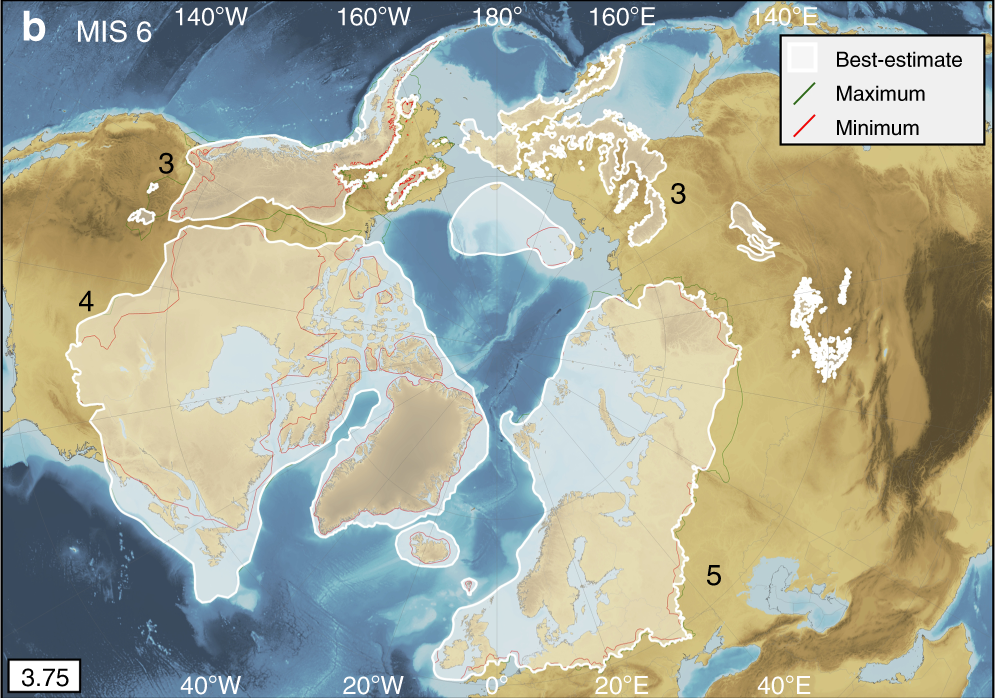
\includegraphics[height=0.76\textheight]{figs/nh-batchelor2019.png}};
  \begin{scope}[x={(map.south east)},y={(map.north west)}]
    \fill[icAccent] (0.494,0.045) circle (1.8pt);
    \node[icAccent,font=\footnotesize\bfseries,anchor=west] at (0.57,0.15) (lon) {London};
    \draw[icAccent,thin] (lon.west) -- (0.494,0.045);
    \fill[icAccent] (0.382,0.762) circle (1.8pt);
    \node[icAccent,font=\footnotesize\bfseries,anchor=west] at (0.45,0.85) (fbk) {Fairbanks};
    \draw[icAccent,thin] (0.45, 0.84) -- (0.382,0.762);
    \fill[icAccent] (0.500,0.503) circle (1.8pt);
    \node[icAccent,font=\footnotesize\bfseries,anchor=west] at (0.57,0.42) (np) {North Pole};
    \draw[icAccent,thin] (np.west) -- (0.500,0.503);
  \end{scope}
\end{tikzpicture}
\end{center}

\vspace{-2mm}
\figcite{best-estimate extent at Marine Isotope Stage 6 ($\sim$140,000 years before present)}

\figcite{Fig.~1b from Batchelor et al (2019), Nature Commun.~10, 3713; added \alert{red} labels}
\end{frame}


\begin{frame}{North American glaciation from 18ka BP to near present}
\centering
\mbox{%
\foreach \n in {1,...,13}{%
  \includegraphics<\n>[height=0.85\textheight,page=\n]{figs/dalton2020-every3.pdf}%
}
% optional: auto-advance in fullscreen mode instead of clicking
%\transduration<1-11>{0.7}
\begin{minipage}{0.3\textwidth}
\grey{\scriptsize from Dalton et al (2020), \par Quaternary Science Reviews 234}
\end{minipage}
}
\end{frame}


\begin{frame}{nearby: British-Irish ice sheet at 26 ka BP}

\centering
\mbox{%
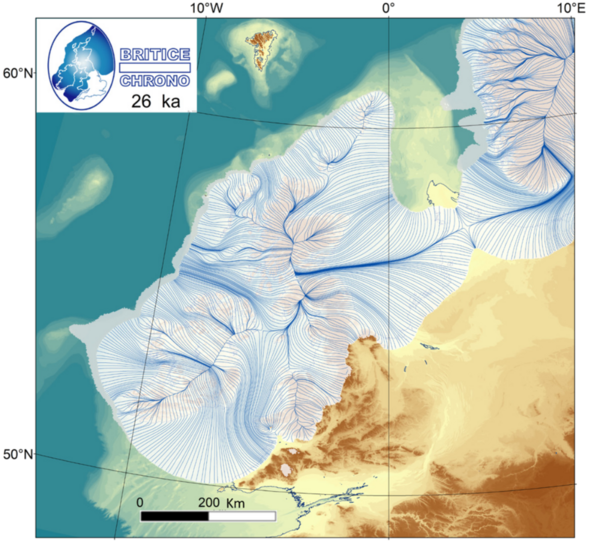
\includegraphics[height=0.8\textheight]{figs/british-clark2022.png} \,
\begin{minipage}{0.3\textwidth}
\grey{\scriptsize Clark et al (2022), Boreas 51}
\end{minipage}
}
\end{frame}


\begin{frame}{glaciers are gravity- and climate-driven flows}

\begin{columns}
\begin{column}{0.5\textwidth}
\only<1>{
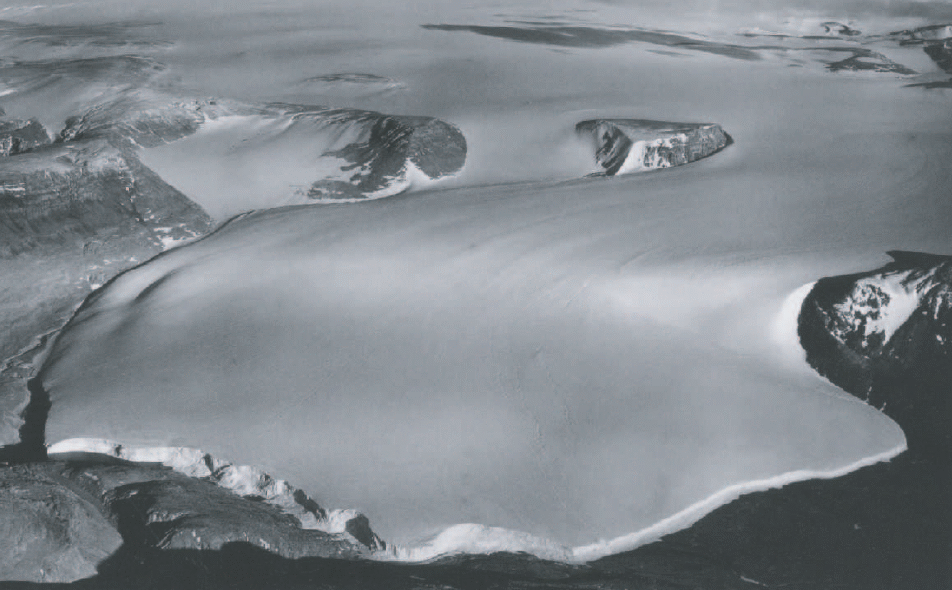
\includegraphics[width=\textwidth]{figs/polaris.png}
\figcite{Polaris Glacier, Greenland; Post \& LaChappelle 2000}
}
\only<2>{
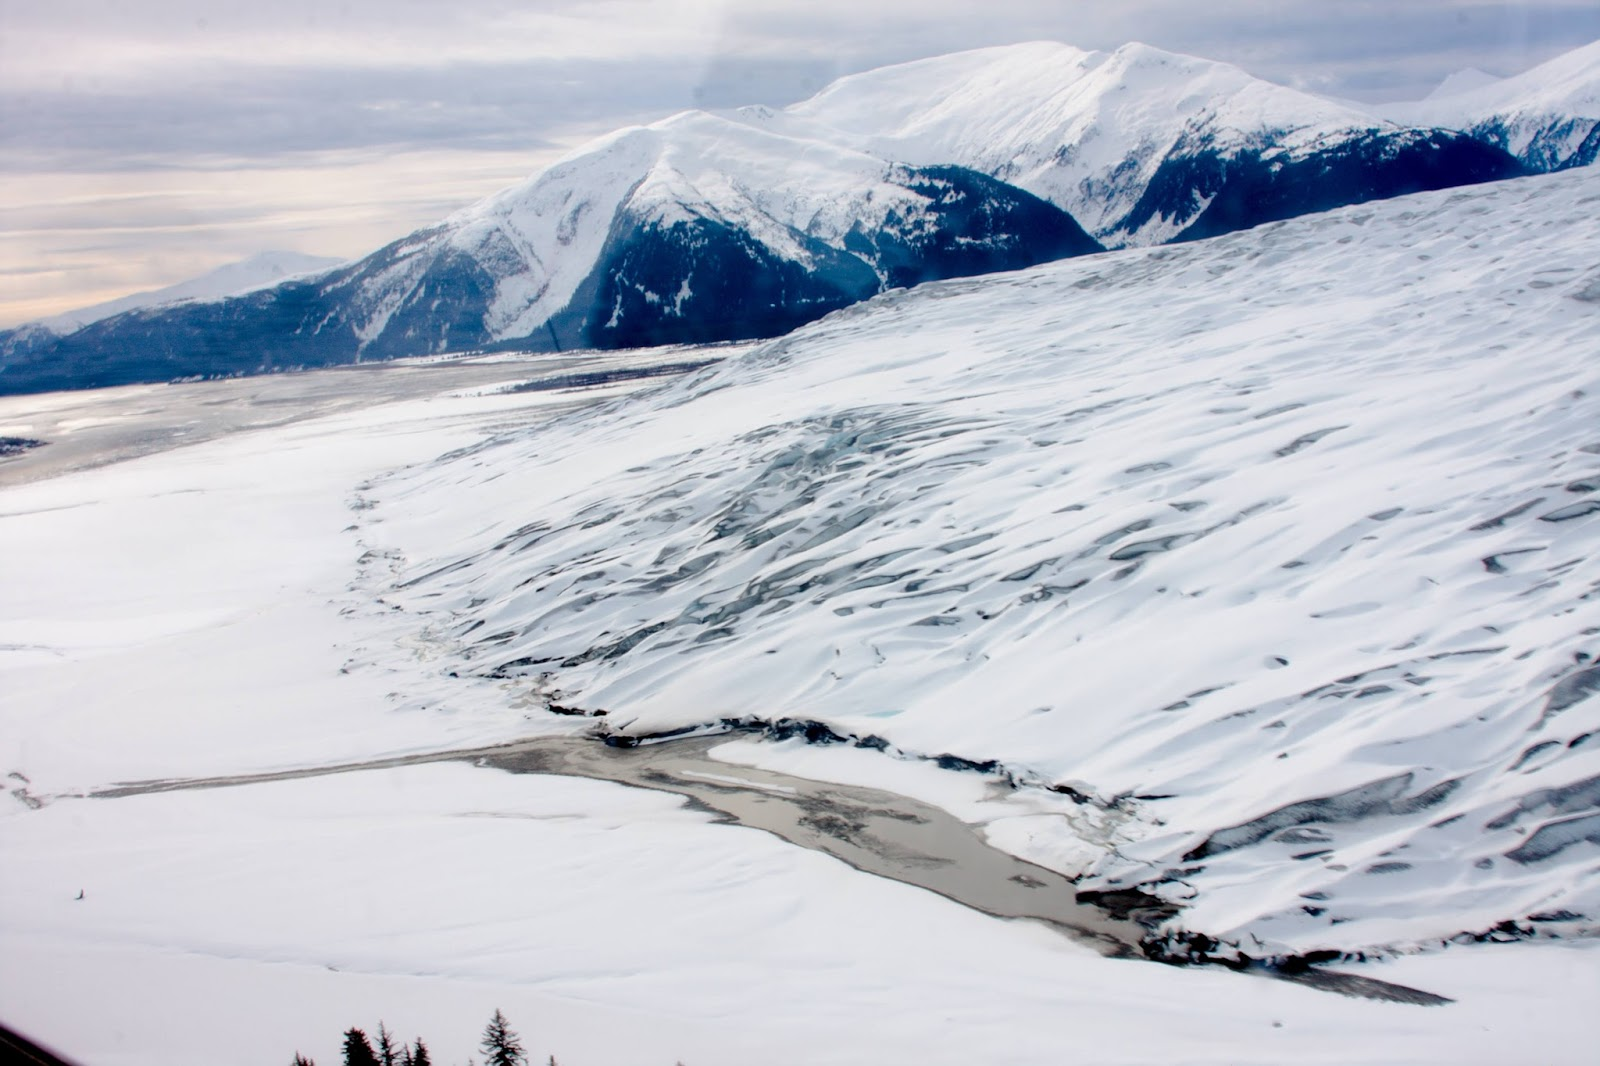
\includegraphics[width=\textwidth]{figs/truffertaku2016.jpg}
\figcite{M.~Truffer photo; Taku Glacier 2016}
}
\end{column}
\begin{column}{0.5\textwidth}
\begin{itemize}
\item a \alert{glacier} is a mass of water ice, as a very-viscous, gravity-driven flow
    \begin{itemize}
    \item[$\circ$] formed from compressed snow
    \item[$\circ$] an \alert{ice sheet} is just a big, continent-scale glacier
    \item[$\circ$] \emph{sea ice is something quite different!}
    \end{itemize}
\item \alert{glaciation} means the glacier-covered, time-dependent 2D domain
\item<2> the \alert{glacier margin} is the free boundary of glaciation
    \begin{itemize}
    \item[$\circ$] location determined by combined effects of climate, bed topography, boundary stresses, and ice flow
    \item[$\circ$] fractures and crevasses \emph{may} dominate margins at small scale
    \item[$\circ$] steeper surface slopes near margins
    \end{itemize}
\end{itemize}
\end{column}
\end{columns}
\end{frame}


\begin{frame}{qualitative observations about ice sheets}

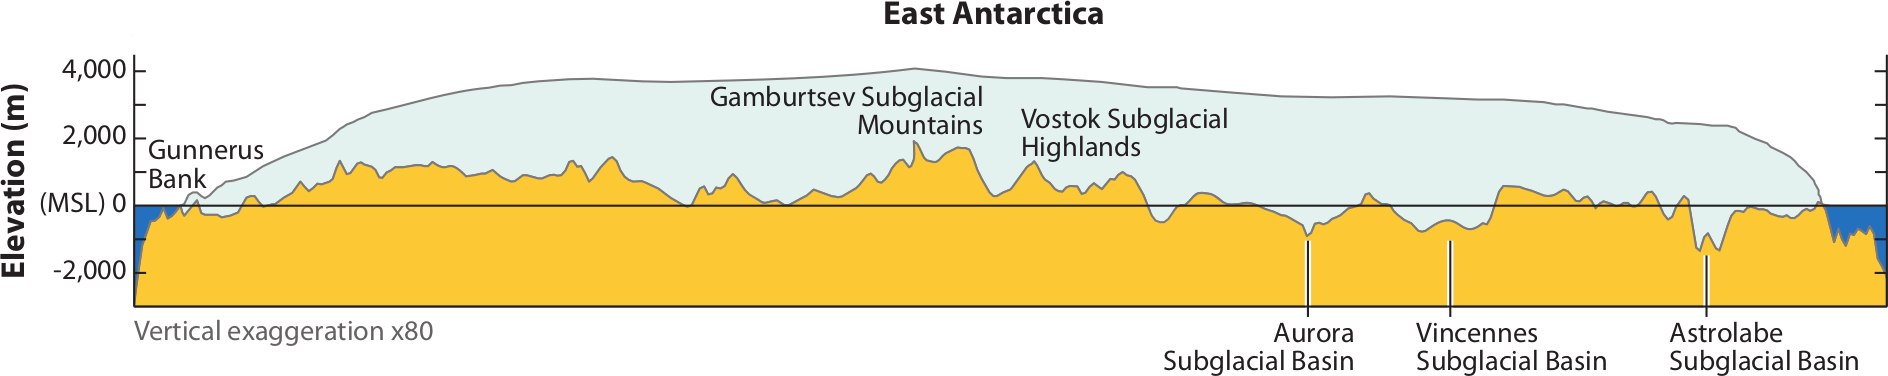
\includegraphics[width=\textwidth]{figs/ant-schoofhewitt2013.png}

\medskip
\figcite{cross-section of East Antarctica, with \alert{80$\times$ vertical exaggeration}}

\figcite{Schoof \& Hewitt (2013), Annu.~Rev.~Fluid Mech.~45, 217--239}

\medskip
\begin{itemize}
\item there are two present-day ice sheets: Antarctica (big!), Greenland (modest)

\pause
\item very thin
\item smooth surface, often above a rough bed
\item steeper surface slopes near margins
\end{itemize}
\end{frame}


\begin{frame}{qualitative observations about ice sheets}

\begin{columns}
\begin{column}{0.6\textwidth}
\hfill 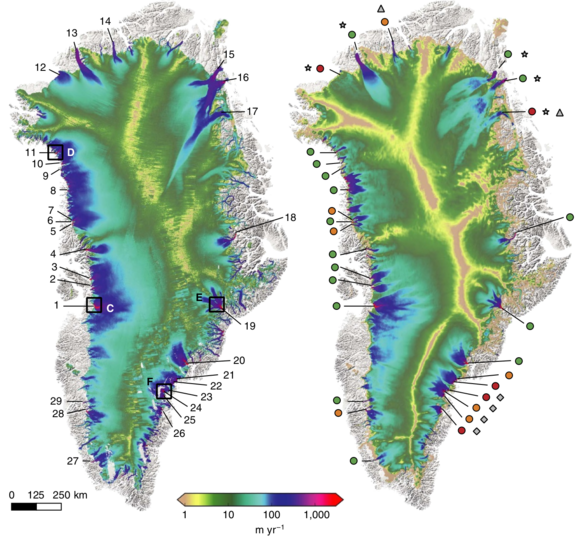
\includegraphics[width=0.93\textwidth]{figs/gis-aschwanden2016.png}
\end{column}
\begin{column}{0.4\textwidth}
\vspace{20mm}

\begin{itemize}
\item large velocity contrasts
\item fast flow concentrated in narrow outlets near boundary
\item near-fractal boundaries
\end{itemize}

\vspace{20mm}
\grey{\scriptsize Greenland surface speed

\alert{left: observed}, \, right: modeled

Aschwanden et al (2016), Nature Commun.~7, 10524

}
\end{column}
\end{columns}
\end{frame}


\AtBeginSection[]
{
  \begin{frame}{outline}
  \tableofcontents[currentsection]
  \end{frame}
}


\section{mathematical problem of glaciation}

\begin{frame}{notation for evolving glacier models}

\hfill\includegraphics<1>[width=0.54\textwidth]{figs/notation1.pdf}%
\includegraphics<2>[width=0.54\textwidth]{figs/notation2.pdf}

\begin{overprint}
\onslide<1>
\vspace{-8mm}

\begin{itemize}
\item fixed land domain \alert{$\Omega\subset\RR^2$}
    \begin{itemize}
    \item[$\lc$] $x = (x_1,x_2) \in \Omega$
    \end{itemize}
\item \alert{surface mass balance} $a(t,x)$ \grey{[m$\,$a$^{-1}$;\, the climate as seen by the glacier]} \hfill \grey{$\leftarrow$ data}
    \begin{itemize}
    \item[$\lc$] $a>0$ is accumulation of snow
    \item[$\lc$] $a<0$ is ablation by melt
    \item[$\lc$] assuming: $a$ is defined everywhere in $\Omega$, \emph{even where there is no ice}
    \end{itemize}
\item \alert{bed elevation} $b(x)$ \grey{[m]} \hfill \grey{$\leftarrow$ data}
    \begin{itemize}
    \item[$\lc$] defined everywhere in $\Omega$
    \end{itemize}
\end{itemize}
\onslide<2>
\begin{itemize}
\vspace{2mm}

\item \alert{surface elevation} $s(t,x)$ \grey{[m]} \hfill \grey{$\leftarrow$ solution}
    \begin{itemize}
    \item[$\lc$] equivalent geometry variable: \alert{thickness} $H(t,x)=s(t,x)-b(x)$
    \item[$\lc$] required:\, $\alert{s(t,x)\ge b(x)} \, \iff \, H(t,x)\ge 0$
    \end{itemize}
\item \alert{ice domain} $\displaystyle \Lambda(t) = \left\{(x,z) \,:\, b(x) < z < s(t,x)\right\} \subset \RR^3$  \hfill \grey{$\leftarrow$ solution}
    \begin{itemize}
    \item[$\lc$] this 3D set is an output, \emph{not data}
    \item[$\lc$] \alert{glaciation} is \, $\Lambda(t)^\perp = \left\{x \,:\, b(x) < s(t,x)\right\} \subset \Omega$, also an output
    \end{itemize}
\end{itemize}
\end{overprint}
\end{frame}


\begin{frame}{surface elevation view: how does the surface move?}

\begin{itemize}
\item \alert{surface kinematical equation}:
\begin{equation*}
\frac{\partial s}{\partial t} + \bu|_s \cdot \bn_s = a
\end{equation*}

    \begin{itemize}
    \item[$\lc$] $\bu|_s$ is the \alert{surface trace of 3D ice velocity} \only<2>{\hfill \grey{$\leftarrow$ solution}}
    \item[$\lc$] $\bn_s = \left<-\tfrac{\partial s}{\partial x_1}, -\tfrac{\partial s}{\partial x_1}, 1\right>$ is the upward \alert{surface normal vector} \only<2>{\hfill \grey{$\leftarrow$ solution}}
    \item[$\lc$] e.g.~apply pillbox mass-conservation argument to derive
    \end{itemize}

\medskip
\pause
\item this equation applies at the \alert{non-material} surface $z=s(t,x)$ \alert{only if  $s(t,x) > b(x)$},
\item so it \alert{cannot}, by itself, describe the evolution of glaciation
\end{itemize}
\end{frame}


\begin{frame}{surface elevation view: advection with inequality constraint}

\hfill 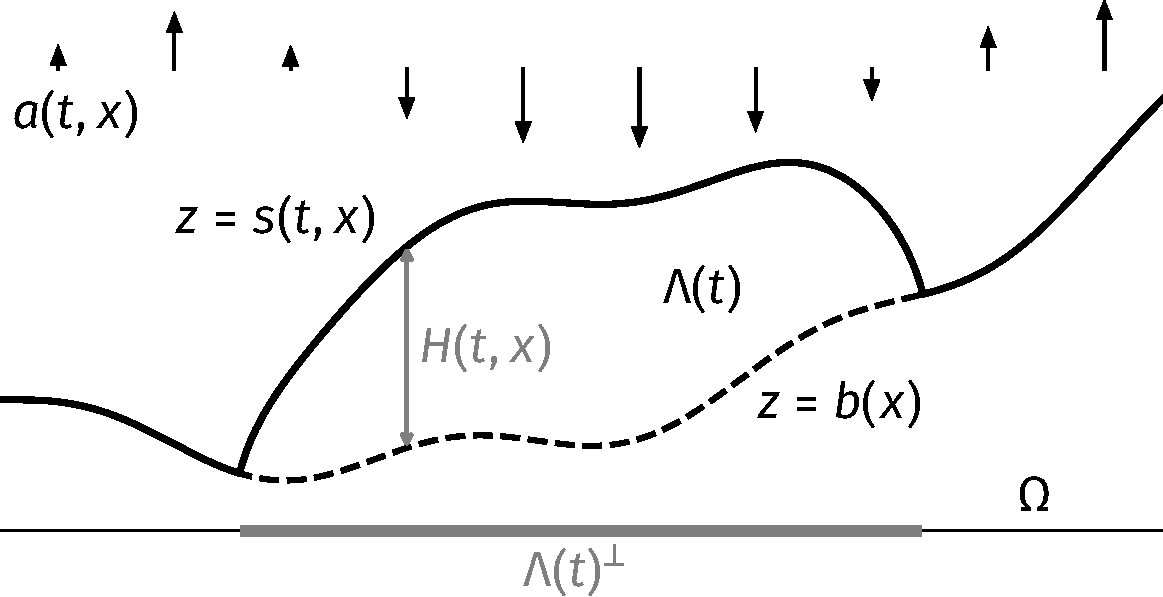
\includegraphics[width=0.35\textwidth]{figs/notation2.pdf}

\vspace{-9mm}
\begin{itemize}
\item Q: how does the glacier and the glaciation \alert{evolve}?
    \begin{itemize}
    \item[$\lc$] for the moment, ignoring the stress balance in $\Lambda(t)$
    \end{itemize}

\pause
\item A: via a \alert{nonlinear complementarity problem} (NCP) on $[0,T]\times\Omega$:
\begin{align*}
s - b &\ge 0 \\
\frac{\partial s}{\partial t} + \bu|_s \cdot \bn_s - a &\ge 0 \\
(s-b) \left(\frac{\partial s}{\partial t} + \bu|_s \cdot \bn_s - a\right) &= 0
\end{align*}

    \begin{itemize}
    \item[$\lc$] assuming: \,\alert{$\bu|_s$ is extended by zero to ice-free land}
    \item[$\lc$] at ice-free locations ($s=b$, $\partial s/\partial t=0$, $\bu|_s=\bzero$) we have $a\le 0$, ablation
    \end{itemize}
\item this is an \alert{obstacle problem}, in strong form, with $b$ as the obstacle
\end{itemize}
\end{frame}


\begin{frame}{thickness view: scalar conservation with inequality constraint}

\hfill 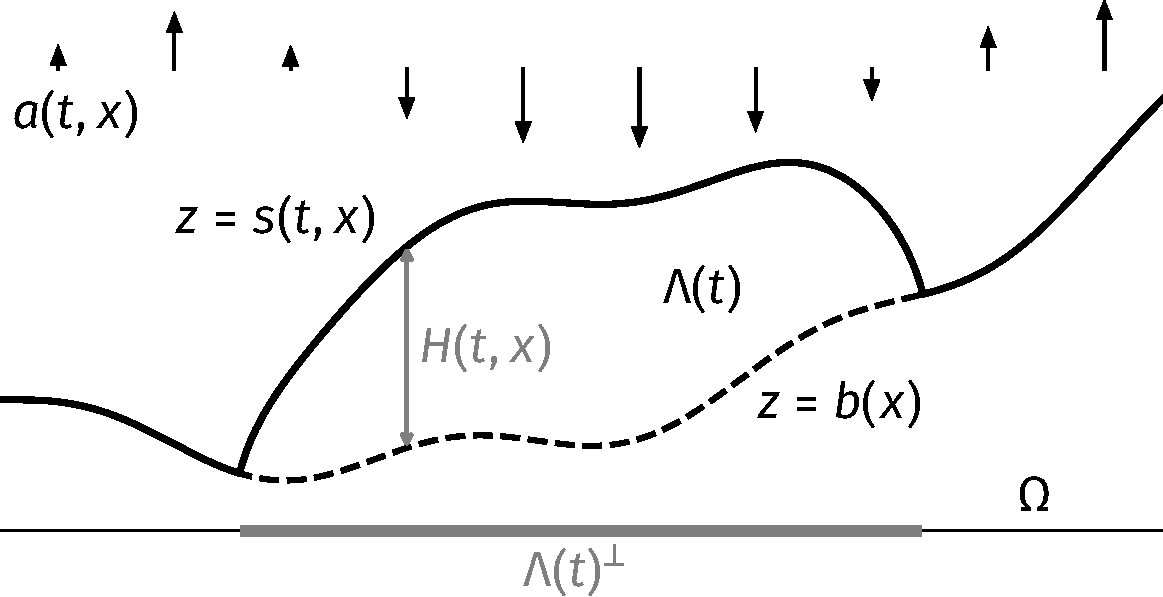
\includegraphics[width=0.35\textwidth]{figs/notation2.pdf}

\vspace{-15mm}
\begin{itemize}
\item there is another view, equally valid,

using thickness $H(t,x)=s(t,x)-b(x)$
\item $\bU=$ (horizontal ice velocity in $\Lambda(t)$)
\item define the \alert{ice flux}:
$$\alert{\bq(t,x)=\int_{b(x)}^{s(t,x)} \bU(t,x,z)\,dz} \hspace{30mm}$$
\item again an NCP, an obstacle problem:

\vspace{-5mm}
{\small
\begin{align*}
H &\ge 0 \\
\frac{\partial H}{\partial t} + \Div\bq - a &\ge 0 \\
H\left(\frac{\partial H}{\partial t} + \Div\bq - a\right) &= 0
\end{align*}
}

    \begin{itemize}
    \item[$\lc$] \alert{where ice is present mass is conserved}: \,$\frac{\partial H}{\partial t} + \Div\bq - a = 0$
    \item[$\lc$] at ice-free locations ($H=0$, $\partial H/\partial t = 0$, $\bq=\bzero$) we have $a\le 0$, ablation
    \end{itemize}
\end{itemize}
\end{frame}


\begin{frame}{why prefer surface elevation?}

\centering
\mbox{%
\hspace{20mm}
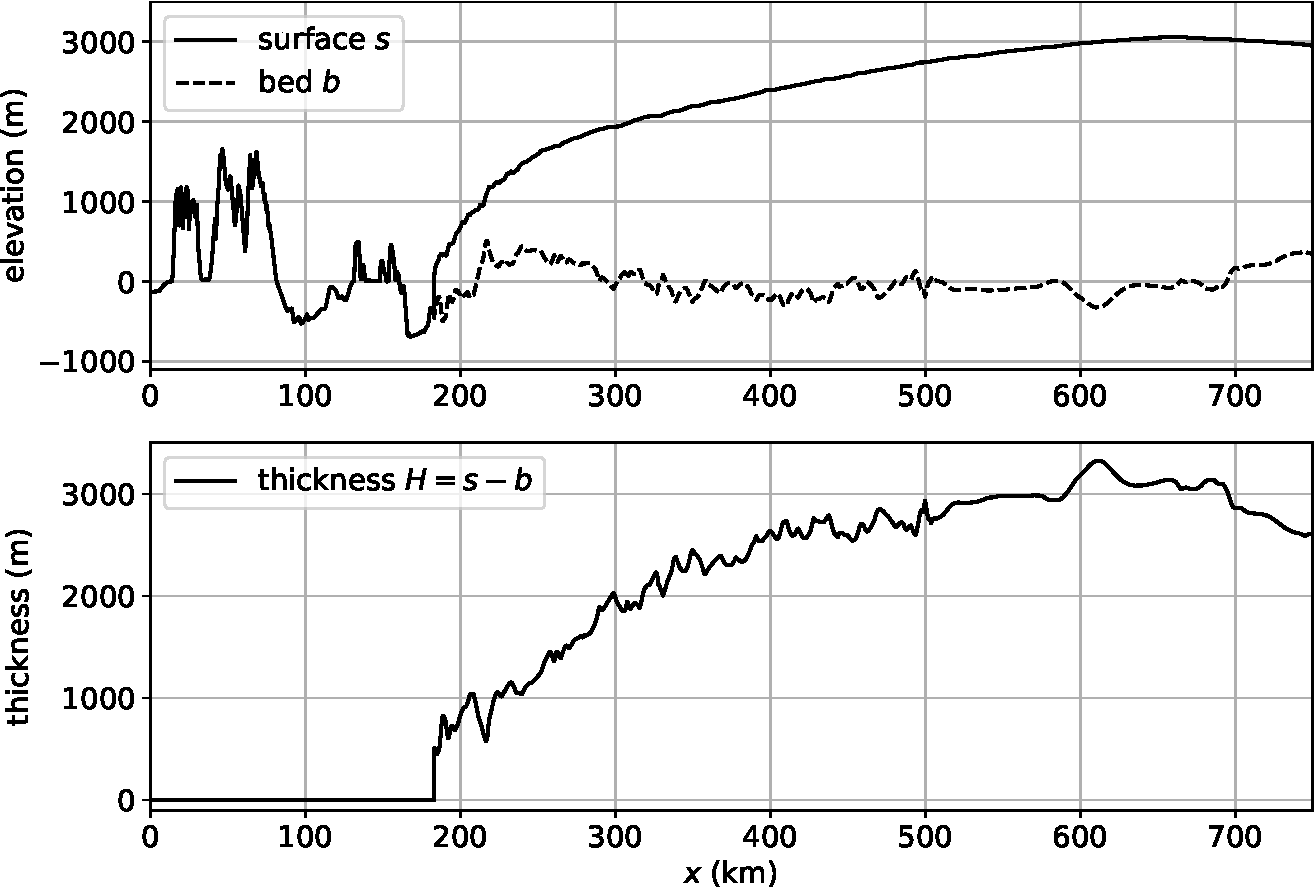
\includegraphics[height=0.56\textheight]{figs/giscross.pdf} \,
\begin{minipage}{0.3\textwidth}
\grey{\scriptsize Greenland cross-section at $70^\circ$N

data from Morlighem et al.~2017}
\end{minipage}
}

\medskip
\begin{itemize}
\item gravity-driven \alert{ice flow} causes the surface $s(t,x)$ to \alert{become smoother}
\item meanwhile $H(t,x)=s(t,x)-b(x)$ inherits the (spatial) low regularity of the bed
\end{itemize}
\end{frame}


\begin{frame}{translation: glaciers $\leftrightarrow$ optimization}

\begin{columns}
\begin{column}{0.63\textwidth}
\begin{itemize}
\item some language from inequality-constrained optimization is useful

\begin{definition}
An inequality constraint ``$f(x)\ge c$'' is \alert{active} on $\{x\,:\,f(x)=c\}$ and \alert{inactive} otherwise, on $\{x\,:\,f(x)>c\}$.
\end{definition}

\medskip
\item<2> for map-plane subsets of $\Omega$, at $t$:
\end{itemize}
\end{column}
\begin{column}{0.37\textwidth}
\hfill \includegraphics<1->[width=\textwidth]{figs/notation2.pdf}

\vspace{10mm}
\vspace{0pt}
\end{column}
\end{columns}

\onslide<2>{
\begin{center}
\begin{tabular}{rcl|c}
glaciology     &                   & optimization  & subset \\ \hline
glaciated area & $\leftrightarrow$ & inactive set  & $\Lambda(t)^\perp${\Large \strut} \\
ice-free area  & $\leftrightarrow$ & active set    & \,\,$\Omega \setminus \Lambda(t)^\perp${\large \strut} \\
glacier margin & $\leftrightarrow$ & free boundary & \,\, $\Omega \cap \partial\Lambda(t)^\perp${\large \strut}
\end{tabular}
\end{center}
}
\end{frame}


\begin{frame}{equivalence: weak surface motion equals weak flux divergence}

\begin{itemize}
\item recall equivalent equations, applying in the inactive set $\Lambda(t)^\perp$:
   $$\frac{\partial s}{\partial t} + \bu|_s \cdot \bn_s = a \qquad \leftrightarrow \qquad \frac{\partial H}{\partial t} + \Div\bq = a$$
\item I will call $-\bu|_s \cdot \bn_s$ the \alert{surface motion}
\end{itemize}

\begin{lemma}
If ice is incompressible and if $\bu|_b\cdot \hat\bn = 0$ then for a test function $\omega(x)$ on $\Omega$:

\hspace{30mm} $\displaystyle \alert{\int_\Omega (\bu|_s\cdot \bn_s)\, \omega \,dx = \int_\Omega \bq \cdot \grad \omega\,dx}$.
\end{lemma}

\pause
{\footnotesize
\noindent \textbf{proof.} \, Extend to $\Lambda(t)\subset \RR^3$:\, $\omega(x)=\tilde\omega(x,z)$.  Recall $\bn_s = \left<-\grad s,1\right>$.  Then
\begin{align*}
\int_\Omega (\bu|_s\cdot \bn_s)\, \omega\,dx &= \int_{\partial\Lambda(t)} \tilde\omega\,\bu\cdot\hat\bn\,ds && \afcomm{only top contributes;\, \alert{$\bn_s\,dx=\hat\bn\,ds$}} \\
&= \int_{\Lambda(t)} \Div\left(\tilde\omega\,\bu\right)\,dx\,dz = \int_{\Lambda(t)} \bu\cdot\grad\tilde\omega\,dx\,dz && \afcomm{div theorem;\, \alert{incompressibility}} \\
&= \int_\Omega \bq \cdot\grad\omega\,dx && \afcomm{$\tilde\omega$ indep of $z$;\, def of $\bq$} \hspace{15mm} \hfill \qed
\end{align*}
}
\end{frame}


\newcommand{\stokesblock}{%
\begin{align*}
-\Div\left(2\nu(D\bu)D\bu\right)+\grad p &= \rhoi\bg && \text{in $\Lambda$} \qquad\qquad\quad \grey{\text{stress balance}} \\
\Div\bu &= 0                                         && \text{in $\Lambda$} \qquad\qquad\quad \grey{\text{incompressible}} \\
\left(2\nu D\bu-pI\right)\bn_s &= \bzero && \text{on $\Gamma_s\subset\partial \Lambda$ \qquad \grey{stress free}} \\
\bu &= \bzero && \text{on $\Gamma_b\subset\partial \Lambda$ \qquad \grey{non-sliding}}
\end{align*}
}

\section{well-posedness, and coercivity confusion}

\begin{frame}{momentum conservation: Stokes on domain $\Lambda(t)$ at fixed $t$}

\begin{itemize}
\item let \alert{$\pp = 1 + 1/\nn \approx 4/3$}, where $\nn\approx 3$ is \alert{Glen's exponent} for ice rheology
\item $D\bu = 0.5 (\grad \bu + \grad \bu^\top)$ is the \alert{strain rate}
\item fix $t$ and consider the ice domain $\Lambda=\Lambda(t)=\{(x,z):b<z<s\}$
\item for the \alert{effective viscosity} $\nu(D\bu)=\nu_0 |D\bu|^{\pp-2}$,
\end{itemize}

\vspace{-4mm}
{\small
\stokesblock
}

\pause
\vspace{-1mm}
\begin{block}{fixed-domain theory \grey{(Jouvet \& Rappaz 2011, for example)}}
if $\Lambda$ is a bounded Lipschitz domain then there is a unique $(\bu,p)\in W^{1,\pp}(\Lambda;\RR^3)\times L^{\pp'}(\Lambda)$ solving the above
\end{block}

\begin{itemize}
\item a surface trace bound applies \pfcomm{B 2026}:\,$\int_{\Gamma_s}\big|\bu|_s\big|^\pp\,dS \le C$
\end{itemize}
\end{frame}


\begin{frame}{the surface-Stokes evolution model?}

{\small
\stokesblock
}

\begin{itemize}
\item let \alert{$\pp = 1 + 1/\nn \approx 4/3$}, where $\nn\approx 3$ is \alert{Glen's exponent} for ice rheology
\item $D\bu = 0.5 (\grad \bu + \grad \bu^\top)$ is the \alert{strain rate}
\item fix $t$ and consider the ice domain $\Lambda=\Lambda(t)=\{(x,z):b<z<s\}$
\item for the \alert{effective viscosity} $\nu(D\bu)=\nu_0 |D\bu|^{\pp-2}$,
\end{itemize}

\vspace{-4mm}
{\small
\begin{align*}
-\Div\left(2\nu(D\bu)D\bu\right)+\grad p &= \rhoi\bg && \text{in $\Lambda$} \qquad\qquad\quad \grey{\text{stress balance}} \\
\Div\bu &= 0                                         && \text{in $\Lambda$} \qquad\qquad\quad \grey{\text{incompressible}} \\
\left(2\nu D\bu-pI\right)\bn_s &= \bzero && \text{on $\Gamma_s\subset\partial \Lambda$ \qquad \grey{stress free}} \\
\bu &= \bzero && \text{on $\Gamma_b\subset\partial \Lambda$ \qquad \grey{non-sliding}}
\end{align*}
}

\pause
\vspace{-1mm}
\begin{block}{fixed-domain theory \grey{(Jouvet \& Rappaz 2011, for example)}}
if $\Lambda$ is a bounded Lipschitz domain then there is a unique $(\bu,p)\in W^{1,\pp}(\Lambda;\RR^3)\times L^{\pp'}(\Lambda)$ with $\bu=\bzero$ on $\Gamma_b$, and a surface trace bound applies \pfcomm{B 2026}:
\,$\int_{\Gamma_s}\big|\bu|_s\big|^\pp\,dS \le C$
\end{block}

\begin{itemize}
\item but the domain is \alert{not} fixed, and the surface is itself the solution
\item no time derivative: Stokes is an \alert{algebraic} constraint on a free-boundary evolution \, $\implies$ \, a differential-algebraic system with inequality constraints, so implicit steps are natural
\end{itemize}
\end{frame}


\subsection{shallow ice approximation}

\begin{frame}{shallow ice approximation (SIA)}

\begin{itemize}
\item as with many fluid properties, the \alert{lubrication approximation} model was first historically
\item scales: $[L]$ horizontal extent, $[H]$ thickness
\item 
\item in the small aspect-ratio limit, with no sliding and isothermal ice, Glen exponent $\nn\approx 3$, the flux is \alert{local}:
    $$\bq = -\Gamma\, H^{\nn+2} |\grad s|^{\nn-1}\grad s, \qquad \Gamma = \frac{2A(\rho g)^\nn}{\nn+2}$$
\item so thickness solves a \alert{degenerate, doubly-nonlinear} obstacle problem:
    $$H\ge 0, \qquad \frac{\partial H}{\partial t} - \Div\left(\Gamma H^{\nn+2} |\grad (H+b)|^{\nn-1}\grad (H+b)\right) - a \ge 0, \qquad \text{complementarity}$$
\item if the bed is flat, the transformation $w=H^{m}$, $m=2(\nn+1)/\nn=8/3$, gives a $\pp$-Laplacian with $\pp=\nn+1=4$:
    $$\frac{\partial}{\partial t}\left(w^{1/m}\right) - \mu \Div\left(|\grad w|^{\pp-2}\grad w\right) - a \ge 0$$
\item if the bed is not flat, there is a solution-dependent ``tilt'': \, $\grad w \to \grad w - \Phi_b(w)$
\item this is the only place where we have well-posedness theorems for glacier geometry
\end{itemize}
\end{frame}


\begin{frame}{shallow ice approximation (SIA): velocity and flux from a formula}

\begin{itemize}
\item in the small aspect-ratio limit, with no sliding and isothermal ice, Glen exponent $\nn\approx 3$, the flux is \alert{local}:
    $$\bq = -\Gamma\, H^{\nn+2} |\grad s|^{\nn-1}\grad s, \qquad \Gamma = \frac{2A(\rho g)^\nn}{\nn+2}$$
\item so thickness solves a \alert{degenerate, doubly-nonlinear} obstacle problem:
    $$H\ge 0, \qquad \frac{\partial H}{\partial t} - \Div\left(\Gamma H^{\nn+2} |\grad (H+b)|^{\nn-1}\grad (H+b)\right) - a \ge 0, \qquad \text{complementarity}$$
\item if the bed is flat, the transformation $w=H^{m}$, $m=2(\nn+1)/\nn=8/3$, gives a $\pp$-Laplacian with $\pp=\nn+1=4$:
    $$\frac{\partial}{\partial t}\left(w^{1/m}\right) - \mu \Div\left(|\grad w|^{\pp-2}\grad w\right) - a \ge 0$$
\item if the bed is not flat, there is a solution-dependent ``tilt'': \, $\grad w \to \grad w - \Phi_b(w)$
\item this is the only place where we have well-posedness theorems for glacier geometry
\end{itemize}
\end{frame}

\begin{frame}{Jouvet \& B (2012): bumpy 2D, steady}

FIXME steady

\begin{withpeople}{\photo[13mm]{figs/people/gjouvet.png}{G.~Jouvet}}
\begin{theorem}[Jouvet \& B 2012]
for $\Omega\subset\RR^2$, $\pp>2$, general bed $b\in W^{1,\pp}(\Omega)$, plus sliding, variable softness, and elevation-dependent $a$, the steady SIA as a VI over $\cK=\{v\in W_0^{1,\pp}(\Omega):v\ge 0\}$,
    $$\int_\Omega \left(\mu(x,w)|\grad w-\Phi_b(x,w)|^{\pp-2}\left(\grad w-\Phi_b(x,w)\right) - \Psi(x,w)\right)\cdot\grad(v-w) \ge \int_\Omega \alpha(x,w)\,(v-w)$$
for all $v\in\cK$, has \alert{at least one solution}, and every solution satisfies $\|w\|_{W^{1,\pp}}<C$
\end{theorem}

\begin{itemize}
\item proof: a fixed point argument; freezing the nonlinearities gives a monotone problem
\item uniqueness in the flat, no-sliding, elevation-independent case (convex minimization)
\item for general beds: \alert{uniqueness left open}
\item steady state corresponds to $\Delta t\to\infty$
\end{itemize}
\end{withpeople}
\end{frame}


\begin{frame}{uniqueness fails for steady states on bumpy beds}

\centerline{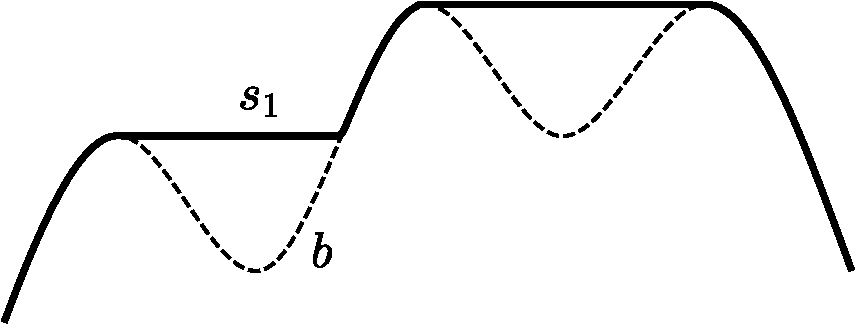
\includegraphics[width=0.38\textwidth]{figs/filled.pdf} \quad 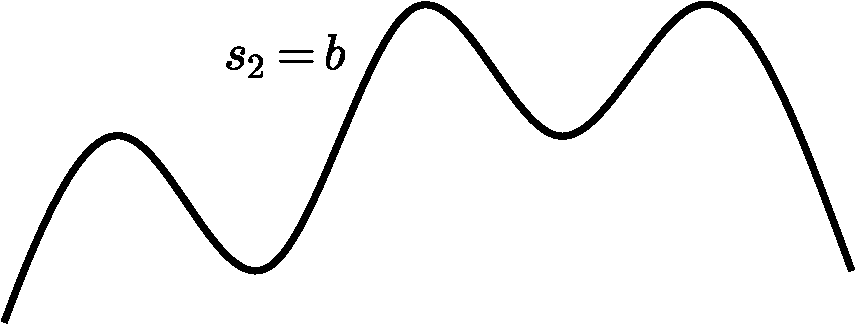
\includegraphics[width=0.38\textwidth]{figs/icefree.pdf}}
\figcite{$s_1$ fills basins with flat ice, $s_2=b$ is ice-free; from B (2026), Appendix B}

\begin{proposition}[B 2026]
let $b$ be smooth with strict local minima, and let $a=0$ on the basins and $a\le 0$ elsewhere; then the steady glacier model, in \alert{any} stress balance for which flat ice does not flow, has more than one solution
\end{proposition}

\begin{itemize}
\item proof: both $s_1,s_2$ have $\bu|_{s_i}=\bzero$, so both solve $s-b\ge 0$, \, $-\bu|_s\cdot\bn_s\ge 0$, \, complementarity
\item resolves the open question, for elevation-\emph{in}dependent climates; generally infinitely many solutions
\item consequence: the surface motion map is \alert{not strictly monotone}
\end{itemize}
\end{frame}


\begin{frame}{Calvo et al (2002): flat 1D, time-dependent}

\begin{withpeople}{\photo[8mm]{../talk2/figs/people/generic.png}{N.~Calvo} \photo[8mm]{../talk2/figs/people/generic.png}{J.~D\'iaz} \photo[8mm]{../talk2/figs/people/generic.png}{J.~Durany} \photo[8mm]{../talk2/figs/people/generic.png}{E.~Schiavi} \photo[8mm]{../talk2/figs/people/generic.png}{C.~V\'azquez}}
\begin{theorem}[Calvo, D\'iaz, Durany, Schiavi, V\'azquez 2002]
on a flat bed in one horizontal dimension, for bounded data $a$ and $w_0$, there is a unique bounded weak solution $w\in L^\pp(0,T;W_0^{1,\pp}(\Omega))$; for no sliding (or spatially-constant sliding) and $H_i=w_i^{1/m}$ we have the comparison
    $$\int_\Omega [H_1(t)-H_2(t)]_+ \le \int_\Omega [H_1(0)-H_2(0)]_+ + \int_0^t\!\!\int_\Omega [a_1-a_2]_+$$
\end{theorem}

\begin{itemize}
\item the first place the problem is posed as an obstacle problem
    \begin{itemize}
    \item[$\lc$] the constraint is enforced by a multivalued term: \, $H_t - (\dots)_x + \beta(H) \ni a$
    \end{itemize}
\item the free boundary is proven to exist: in a strongly-ablating region, far enough from accumulation, $H=0$ after some time
\item \alert{waiting time} property: a margin can stay put for a while, until its slope rebuilds
\end{itemize}
\end{withpeople}
\end{frame}


\begin{frame}{Piersanti \& Temam (2023): flat 2D, time-dependent}

\begin{withpeople}{\photo{figs/people/ppiersanti.png}{P.~Piersanti} \photo{figs/people/rtemam.jpg}{R.~Temam}}
\begin{theorem}[Piersanti \& Temam 2023]
for $\Omega\subset\RR^2$ and $2.8\le\pp\le 5$, under the assumptions below, a time-dependent VI over $\cK=\{v\in W_0^{1,\pp}(\Omega):v\ge 0\}$ has a solution, by a semi-discrete scheme and penalty method
\end{theorem}

\medskip
\begin{itemize}
\item ordinary assumptions: flat bed, no sliding, height-independent $A$ and $a$
\item \alert{less ordinary:} a ``decrease condition'' on the \alert{iterates of the penalized scheme}, for all $N\ge 1$:
    $$\left\{w_{\ell}^{n+1,k}\right\}_- \ge \left\{w_{\ell}^{n,k}\right\}_-$$
    \begin{itemize}
    \item[$\lc$] not on data; the authors associate it to a regime of pure melting
    \item[$\lc$] also a regularity condition on the penalized solutions
    \item[$\lc$] the authors: not clear whether existence holds without these
    \end{itemize}
\item uniqueness, continuous dependence, regularity: deferred to future work
\end{itemize}
\end{withpeople}
\end{frame}


\begin{frame}{summary of SIA well-posedness}

\begin{center}
\setlength{\tabcolsep}{5pt}
\begin{tabular}{llllll}
\toprule
 & domain & bed & time & existence & uniqueness \\
\midrule
Calvo et al (2002) & 1D & flat & dependent & yes & yes \\
Piersanti \& Temam (2023) & 2D & flat & dependent & \alert{yes$^*$} & not addressed \\
Jouvet \& B (2012) & 2D & general & steady & yes & only flat case \\
B (2026), App.~B & any & bumpy & steady & -- & \alert{no} \\
\bottomrule
\end{tabular}
\end{center}

\vspace{-2mm}
{\hfill \footnotesize \alert{$^*$} assumes a condition on the iterates of the scheme}

\bigskip
\begin{itemize}
\item open: time-dependent SIA on a general bed \pfcomm{to my knowledge}
\item conceptual question: if the steady problem is not unique, what is the good statement at finite $\Delta t$?
    \begin{itemize}
    \item[$\lc$] the mass term $\int_\Omega s\,\omega$ in an implicit step might help
    \end{itemize}
\item but real ice sheets are not shallow everywhere, and no such theory exists for Stokes
\end{itemize}
\end{frame}


\subsection{surface-Stokes}

\begin{frame}{thickness form: an implicit step is a VI}

\begin{itemize}
\item apply backward Euler, with $a^n$ the average climate over the step
\end{itemize}

\begin{definition}[B 2021]
let $\cX=W_0^{1,p}(\Omega)$ and $\cK=\{\eta\in\cX : \eta\ge 0\}$; the \alert{time-step problem} seeks $H^n\in\cK$ so that
    $$\int_\Omega \left(H^n - H^{n-1} - \Delta t\, a^n\right)(\eta-H^n) \alert{\,-\, \Delta t \int_\Omega \bq(H^n)\cdot\grad(\eta-H^n)} \ge 0 \quad \text{for all } \eta\in\cK$$
\end{definition}

\begin{itemize}
\item the margin \alert{is not an input}, and the stress balance is hidden in the flux term
\end{itemize}

\begin{theorem}[B 2021]
suppose $\bq=\bq(\grad v,v,x)$ is a \alert{local} flux, with standard assumptions, and $a^n$ does not depend on thickness; if for some $c>0$, $r>1$,
\,$\int_\Omega \left(\bq(v)-\bq(w)\right)\cdot\grad(v-w) \le -c\|v-w\|_{W^{1,p}}^r$ on $\cK$,
then the problem has a unique solution
\end{theorem}
\end{frame}


\begin{frame}{surface elevation form: an implicit step is also a VI}

\begin{itemize}
\item the surface kinematical equation (SKE) says that the surface is moved by the ice velocity and the climate:
    $$\frac{\partial s}{\partial t} - \bu|_s\cdot\bn_s - a = 0 \qquad \bn_s=\left<-\grad s,1\right>$$
\item extend the surface velocity trace $\bu|_s$ by zero to bare ground; again the complete statement is an NCP: \quad $s-b\ge 0$, \quad residual $\ge 0$, \quad product $=0$
\end{itemize}

\begin{definition}[B 2026]
let $\cK=\{\sigma\in\cX : \sigma\ge b \text{ and } \sigma|_{\partial\Omega}=b|_{\partial\Omega}\}$ and $\ell^n=s^{n-1}+\Delta t\,a^n$; the \alert{implicit time-step problem} seeks $s=s^n\in\cK$ so that
    $$\int_\Omega \left(s - \Delta t\,\bu|_s\cdot\bn_s - \ell^n\right)(\sigma-s) \ge 0 \quad \text{for all } \sigma\in\cK$$
\end{definition}

\begin{itemize}
\item derivation: on $\{s>b\}$ the integrand is zero; on $\{s=b\}$ the residual $b-\ell^n$ and $\sigma-b$ are both $\ge 0$
\end{itemize}
\end{frame}


\begin{frame}{the Stokes implicit-step problem}

\begin{itemize}
\item $\Phi:\cK\to\cX'$ means: Stokes on $\Lambda(b,s)$, then the trace, then multiply by $\bn_s$; this is well-defined for $\cX=W^{1,\rr}(\Omega)$ with \alert{$2<\rr\le\infty$}
\end{itemize}

\begin{definition}[B 2026]
$F_{\Delta t}(s)[\omega]=\Delta t\,\Phi(s)[\omega]+\int_\Omega s\,\omega$; the \alert{implicit time-step problem} seeks $s\in\cK\subset\cX$ so that
    $$F_{\Delta t}(s)[\sigma-s]\ge\ell^n[\sigma-s] \quad \text{for all } \sigma\in\cK$$
\end{definition}

\begin{itemize}
\item simultaneously determines the \alert{extent}, the \alert{surface elevation}, and the \alert{velocity and pressure}
\item \alert{conjecture:} $\bu|_s$ is Lipschitz in $s$ on bounded subsets of $\cK$
\item the choice of $\rr$ is really about margin shape, where viscous theory is doubtful:
\end{itemize}

\centerline{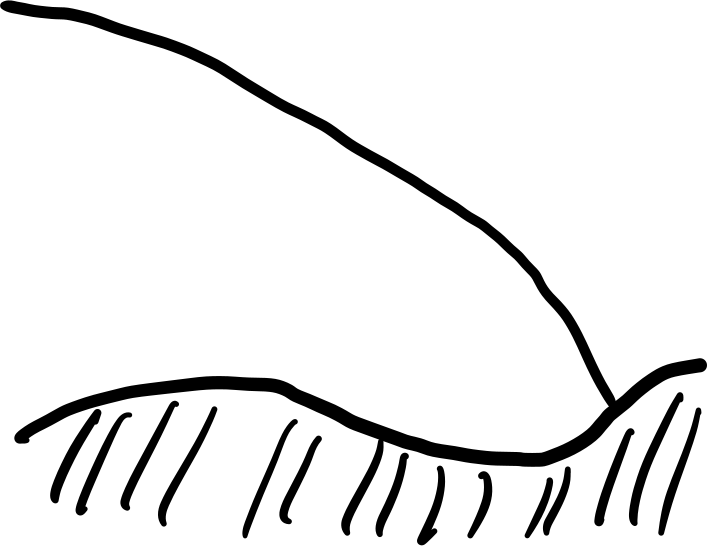
\includegraphics[height=12mm]{figs/wedge.png} \qquad 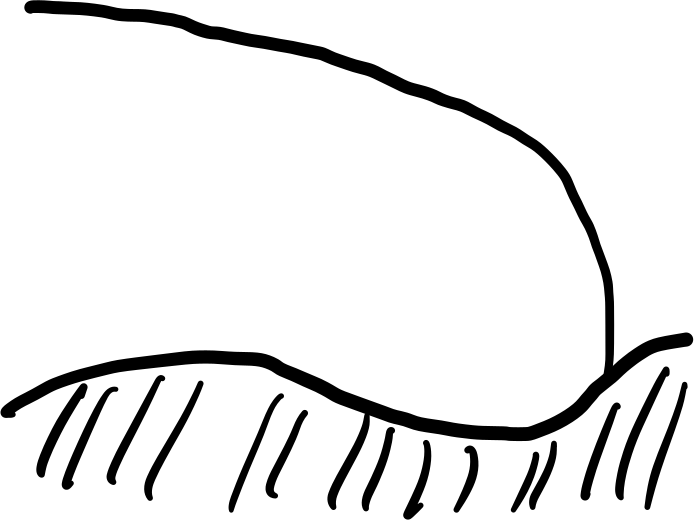
\includegraphics[height=12mm]{figs/unbounded.png} \qquad 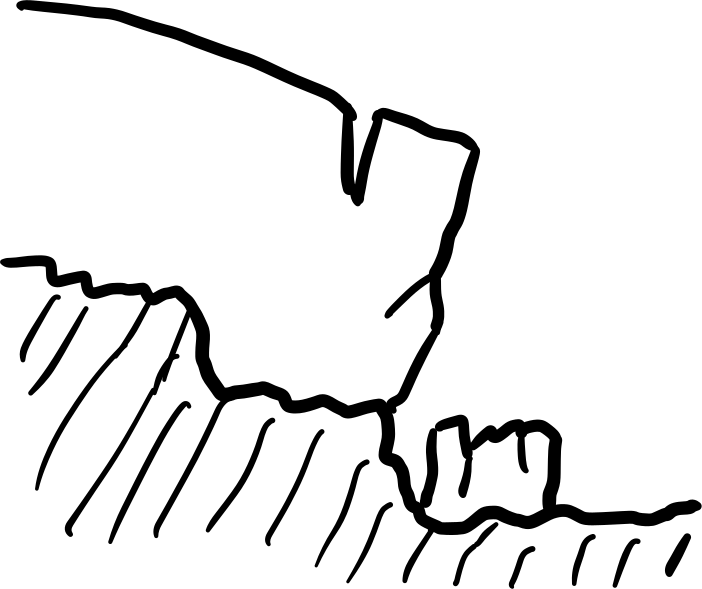
\includegraphics[height=12mm]{figs/realistic.png}}
\figcite{wedge margin; fractional-power margin from shallow theory; real margins overhang and fracture; from B (2026)}
\end{frame}


\begin{frame}{the coercivity question}

\begin{definition}
$f:\cK\to\cX'$ is \alert{$\qq$-coercive} if there is $\alpha>0$ so that $\left(f(v)-f(w)\right)[v-w]\ge\alpha\|v-w\|^\qq$ for all $v,w\in\cK$
\end{definition}

\begin{itemize}
\item bad news: for a bed with local minima, $\Phi$ is \alert{not} $\qq$-coercive for any $\qq$ \pfcomm{Appendix B}
\item good news, heuristically: by the flux form,
    $$\left(\Phi(\sigma)-\Phi(s)\right)[\sigma-s] = -\int_\Omega \left(\bq(\sigma)-\bq(s)\right)\cdot\grad(\sigma-s)$$
    and ice flows downhill: $\bq(s)\sim-\grad s$, \, thus
    $$\left(\Phi(\sigma)-\Phi(s)\right)[\sigma-s]\sim\int_\Omega|\grad\sigma-\grad s|^2$$
    \begin{itemize}
    \item[$\lc$] the rheology does not appear in this reasoning
    \end{itemize}
\item is $\Phi$ \alert{nearly} coercive? \, nothing in a usual statement of Stokes says so
\end{itemize}
\end{frame}


\begin{frame}{numerical experiment on surface pairs (Appendix C)}

\begin{itemize}
\item sample actual surface pairs, and compute the ratios
    $$\rho^0(\sigma,s)=\frac{\left(\Phi(\sigma)-\Phi(s)\right)[\sigma-s]}{\|\sigma-s\|_{W^{1,4}}^4}$$
\item 1D domain: $\Omega=(-100,100)$ km; beds are \emph{flat} and \emph{rough}
\end{itemize}

\centerline{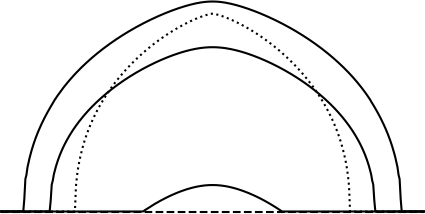
\includegraphics[width=0.32\textwidth]{figs/snapsflat.png} \quad 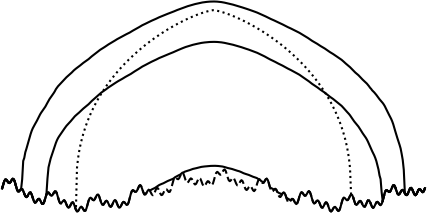
\includegraphics[width=0.32\textwidth]{figs/snapsrough.png}}
\figcite{from B (2026)}

\begin{itemize}
\item $P_1$ surfaces $s_h$; $Q_2\times Q_1$ Stokes on extruded meshes; $\Delta x=500$ m with 40 elements per column
\item surface pairs from 200 year runs: Halfar initial shape, 3 constant SMB values
    \begin{itemize}
    \item[$\lc$] advance and retreat, up to complete disappearance; 1000 random pairs for each bed
    \end{itemize}
\end{itemize}
\end{frame}


\begin{frame}{unregularized ratios: nearly coercive}

\centerline{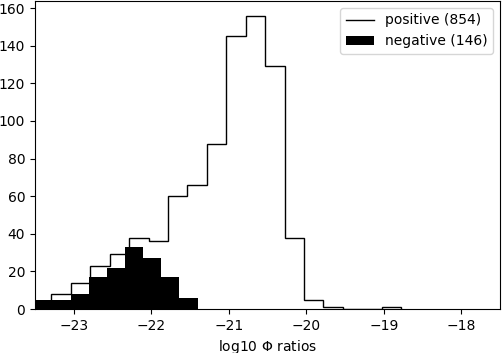
\includegraphics[width=0.56\textwidth]{figs/brough500mNOREG.png}}
\figcite{ratios $|\rho^0(\sigma,s)|$ for the rough bed; from B (2026), Appendix C}

\begin{itemize}
\item about \alert{15\% of ratios are negative} (146 of 1000), which violates coercivity \dots
\item \dots but their magnitudes are \alert{an order of magnitude smaller} than the positive ratios
\item Stokes glacier evolution seemingly ``wants'' to be coercive
\end{itemize}
\end{frame}


\begin{frame}{regularize by a little shallow-ice diffusion}

\begin{itemize}
\item for a fixed thickness $\eta_0>0$ and $0<\eps\ll 1$, using SIA with $\nn=3$, define
    $$\Phi^\eps(s)[\omega]=(1-\eps)\Phi(s)[\omega]+\eps\,\Gamma\eta_0^{5}\int_\Omega|\grad s|^{2}\grad s\cdot\grad\omega \qquad \text{\pfcomm{$4$-Laplacian}}$$
\end{itemize}

\begin{conjecture}[B 2026]
on $\cK\subset\cX=W^{1,4}(\Omega)$ there are $\eps\in(0,1)$, $\eta_0>0$, and $\alpha>0$ so that
    $$\left(\Phi^\eps(\sigma)-\Phi^\eps(s)\right)[\sigma-s]\ge\alpha\|\sigma-s\|_\cX^4 \quad \text{for all } \sigma,s\in\cK$$
\end{conjecture}

\begin{theorem}[B 2026]
assume the two conjectures; then for any $\Delta t>0$ and $s^{n-1}\in\cK$ the regularized implicit time-step VI, with operator $F^\eps_{\Delta t}(s)[\omega]=\Delta t\,\Phi^\eps(s)[\omega]+\int_\Omega s\,\omega$, has a \alert{unique} solution $s\in\cK$
\end{theorem}

\begin{itemize}
\item proof: Lipschitz and $4$-coercive; apply Kinderlehrer \& Stampacchia (1980), Cor.~III.1.8
\item says nothing about time-dependent well-posedness or about $\Delta t\to 0$
\end{itemize}
\end{frame}


\begin{frame}{regularized ratios: credibly coercive}

\centerline{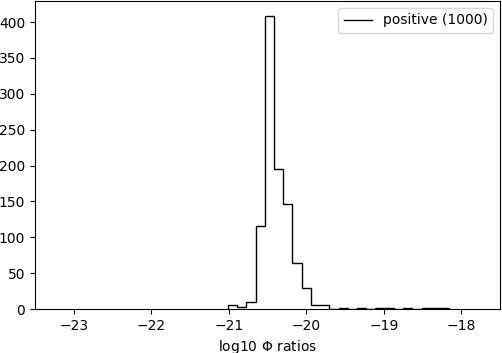
\includegraphics[width=0.56\textwidth]{figs/brough500mREG.png}}
\figcite{ratios $\rho^{0.01}(\sigma,s)$ for the rough bed; from B (2026), Appendix C}

\begin{itemize}
\item with $\eps=0.01$ and $\eta_0=500$ m, \alert{all ratios are positive}, and $\alpha=10^{-22}$ is credible
\item the regularization does not need to do much work
\end{itemize}
\end{frame}


\begin{frame}{consequence: \emph{a priori} bound on an implicit step}

\begin{itemize}
\item $P_1$ surfaces with $b_h\ge b$, so $\cK_h\subset\cK$; \, $\bu_h$ from \emph{any} numerical Stokes solve on $\Lambda(b_h,s_h)$
\end{itemize}

\begin{theorem}[B 2026]
assume the conjectures, and that $s\in\cK$, $s_h\in\cK_h$ solve the regularized VI and its FE version; let $\Pi_h$ be interpolation with truncation into $\cK_h$, and $Z=\left(1+C_\infty[L]^{-1}\|s_h\|_\cX\right)\big\|\bu_h|_{s_h}-\bu|_{s_h}\big\|_{L^{4/3}}$; then with $e_h=s_h-s$,
\begin{align*}
\frac{\alpha\Delta t}{4}\|e_h\|_\cX^4+\frac{1}{2}\|e_h\|_{L^2}^2 &\le \Delta t\int_{\Omega_A(s)}(\Pi_h(s)-b)\,d\nu_s && \text{\alert{[bed and margin]}} \\
&\quad + \Delta t\left(\tfrac{3}{4}\alpha^{-1/3}Z^{4/3}+Z\|\Pi_h(s)-s\|_\cX\right) && \text{\alert{[Stokes solve]}} \\
&\quad + \Delta t\,C\|\Pi_h(s)-s\|_\cX^{4/3}+\frac{1}{2}\|\Pi_h(s)-s\|_{L^2}^2 && \text{\alert{[C\'ea]}}
\end{align*}
\end{theorem}

\begin{itemize}
\item $\nu_s$ is the positive residual measure, on the ice-free set $\Omega_A(s)$; \, proof extends Falk (1974) to nonlinear $F$
\end{itemize}
\end{frame}


\begin{frame}{what the three terms say}

\centerline{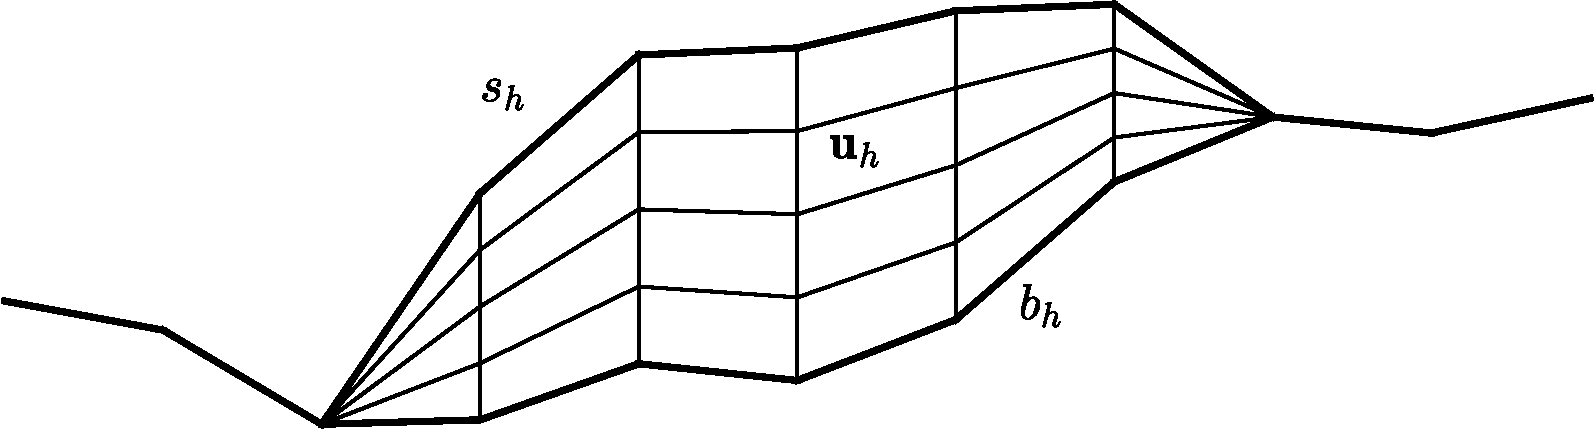
\includegraphics[width=0.5\textwidth]{figs/extruded.pdf}}
\figcite{from B (2026)}

\begin{itemize}
\item \alert{bed and margin:} error in the \alert{unknown ice-free region}, weighted by ablation
    \begin{itemize}
    \item[$\lc$] far from ice, $b_h$ can simply be declared the bare land
    \item[$\lc$] near the exact margin, an inaccurate bed sets an error floor, however good the solver
    \end{itemize}
\item \alert{Stokes solve:} only the \alert{surface trace} error on the numerical domain matters
\item \alert{C\'ea:} interpolation error in $s$, including truncation into $\cK_h$
\item all reduced by refinement, but a \alert{rate} is hard: $s\in W^{2,\mu}$ would need a margin tangent to the bed
\end{itemize}
\end{frame}


\section{state of play: explicit vs implicit}

\begin{frame}{the $L^2$ bound of Tominec et al (2026)}

\begin{withpeople}{\photo[9mm]{figs/people/itominec.jpg}{I.~Tominec} \photo[9mm]{figs/people/llundgren.jpg}{L.~Lundgren} \photo[9mm]{figs/people/alofgren.jpg}{A.~L\"ofgren} \photo[9mm]{figs/people/jahlkrona.png}{J.~Ahlkrona}}
\begin{theorem}[Tominec, Lundgren, L\"ofgren, Ahlkrona 2026]
if $s>b$ and $\bu$ solve the coupled Stokes and free-surface problem, then
    $$\frac{1}{2}\frac{\partial}{\partial t}\|s\|_{L^2}^2=-\frac{2}{\rho g}\|\sqrt{\mu}\,D\bu\|_{L^2(\Lambda(t))}^2+(a,s), \quad \text{thus} \quad \|s(t)\|_{L^2}\le\|s_0\|_{L^2}+\int_0^t\|a\|_{L^2}$$
\end{theorem}

\begin{itemize}
\item proof: test Stokes with $\bu$, and the surface equation with $s$
\item my reading, combining with the flux form: for any admissible $s$,
    $$\Phi(s)[s]=\alert{-\int_\Omega\bq(s)\cdot\grad s}=\frac{1}{\rho g}\int_{\Lambda}2\nu|D\bu|^2\ge 0$$
so ice \alert{provably flows downhill, on average}
\item but: $L^2$ only, assumes $s>b$, and \alert{no control of Stokes domain regularity}
\end{itemize}
\end{withpeople}
\end{frame}


\begin{frame}{the \texttt{stage4/} solver \pcomm{recall lecture 3}}

\begin{withpeople}{\photo[9mm]{figs/people/itominec.jpg}{I.~Tominec} \photo[9mm]{figs/people/alofgren.jpg}{A.~L\"ofgren} \photo[9mm]{figs/people/jahlkrona.png}{J.~Ahlkrona} \photo[9mm]{figs/people/chelanow.png}{C.~Helanow}}
\begin{enumerate}
\item Stokes on the \alert{current} geometry, with a \alert{load stabilization} \pfcomm{L\"ofgren 2022; Tominec 2026 (4.28)}:
    $$\int_{\Lambda^k}2\nu\,D\bu:D\bv-p\Div\bv-q\Div\bu-\rho\bg\cdot\bv+\alert{\int_{\Gamma_s^k}\rho g\Delta t\left[\tfrac{1}{2}\bu\cdot\bn_{s^k}+a\right]\bv\cdot\hat\bn}=0$$
\item surface update as a \alert{VI}, with implicit \alert{edge stabilization} \pfcomm{Tominec 2026 (4.3)}: find $s^{k+1}\in\cK_h$,
    $$\int_\Omega\left(\frac{s^{k+1}-s^k}{\Delta t}-\bu|_{s^k}\cdot\bn_{s^k}-a\right)(\sigma-s^{k+1})+J\left(s^{k+1},\sigma-s^{k+1}\right)\ge 0$$
    with \, $J(s,r)=\sum_e\int_e\tfrac{1}{2}h_e^2\big|\bu|_{s^k}\big|\jump{\grad s}\jump{\grad r}\,dS$
\item choose $\Delta t=C_{\text{CFL}}\min h/|\bu|$ when margins move \pfcomm{$C_{\text{CFL}}=0.25$}
\end{enumerate}


\medskip
\begin{itemize}
\item \alert{split}: only one Stokes solve per step; the VI step is cheap
\end{itemize}
\end{withpeople}
\end{frame}


\begin{frame}{what \texttt{stage4/} does: proof and practice}

\begin{proposition}[Tominec et al 2026: stability of the scheme, if $s^{k+1}>b$]
\vspace{-3mm}
    $$\|s^{k+1}\|_{L^2}^2+\frac{4\Delta t}{\rho g}\|\sqrt{\mu}D\bu\|_{L^2}^2+2\Delta t\,J(s^{k+1},s^{k+1})\le\|s^k\|_{L^2}^2+2\Delta t(a,s^k)+\Delta t^2\|a\|_{L^2}^2$$
\end{proposition}

\medskip
\begin{itemize}
\item with walls ($s>b$): \alert{arbitrary time steps are stable}; without the load term, runs needed $\Delta t\le 0.125$--$0.25$ a

\medskip
\item with moving margins: the VI gives the extent, but velocity is explicit, so \alert{advance is at most one element per step}
    \begin{itemize}
    \item[$\lc$] without the CFL limit: not obviously unstable, but the margin shape is wrong
    \item[$\lc$] with it: ice area drifts about 1\% over 5 years, which is a moving margin effect
    \end{itemize}
\end{itemize}
\end{frame}


\begin{frame}{performance analysis: the setting}

\begin{itemize}
\item parameters \pfcomm{B 2023}:
    \begin{itemize}
    \item[$\lc$] $\Delta x\to 0$ is the map-plane resolution and $m\sim L^2/\Delta x^2$ the number of map-plane nodes
    \item[$\lc$] $q$ is time steps per year needed for ice-climate coupling; $U$ a speed and $D$ an SIA diffusivity
    \item[$\lc$] one Stokes solve is $O(m^{1+\alpha})$ flops; one coupled implicit Stokes step is $O(m^{1+\gamma})$; one implicit SIA step is $O(m^{1+\beta})$
    \end{itemize}
\item stability sets the number of steps per year:
\end{itemize}

\begin{center}
\begin{tabular}{ll}
\toprule
explicit SIA, and \emph{pessimistic} Stokes & $\Delta t<O(D^{-1}\Delta x^2)$ \\
\emph{optimistic} Stokes (advective) & $\Delta t<O(U^{-1}\Delta x)$ \\
implicit: \alert{unconditional}, so only climate limits & $\Delta t<O(q^{-1})$ \\
\bottomrule
\end{tabular}
\end{center}

\begin{itemize}
\item \alert{implicit} means no aspect of geometry or velocity is held fixed in the coupled solve, including the extent
\item (flops per model year) $=$ (steps per year) $\times$ (flops per step)
\end{itemize}
\end{frame}


\begin{frame}{performance analysis: the scaling}

\begin{center}
\begin{tabular}{lll}
\toprule
time-stepping & dynamics & flops per model year \\
\midrule
explicit & SIA & $O\left(D L^2\,\Delta x^{-4}\right)$ \\
explicit & Stokes (optimistic) & $O\left(U L^{2+2\alpha}\,\Delta x^{-(3+2\alpha)}\right)$ \\
explicit & Stokes (pessimistic) & $O\left(D L^{2+2\alpha}\,\Delta x^{-(4+2\alpha)}\right)$ \\
implicit & SIA & $O\left(q L^{2+2\beta}\,\Delta x^{-(2+2\beta)}\right)$ \\
implicit & Stokes & $O\left(q L^{2+2\gamma}\,\Delta x^{-(2+2\gamma)}\right)$ \\
\bottomrule
\end{tabular}
\end{center}
\figcite{Table 2 in B (2023)}

\begin{itemize}
\item explicit Stokes with direct linear algebra ($\alpha\approx 1$) has a horrific $\Delta x^{-5}$ to $\Delta x^{-6}$
\item an existing implicit SIA solver has $\beta=0.8$, so $\Delta x^{-3.6}$; \, implicit constants are large
\item goal: \alert{$\gamma<1/2$ implicit Stokes, thus $O(\Delta x^{-3})$}, better than explicit SIA, presumably by multigrid
    \begin{itemize}
    \item[$\lc$] this is ``an appropriate goal for coming decades''
    \end{itemize}
\end{itemize}
\end{frame}


\begin{frame}{better news from the stabilized solver}

\begin{itemize}
\item a stabilized split scheme does \alert{one fixed-geometry Stokes solve per step}, so $\alpha$ applies, and not $\gamma$:
\end{itemize}

\begin{center}
\begin{tabular}{lll}
\toprule
stabilized, split & case & flops per model year \\
\midrule
fixed extent (proven if $s>b$) & $\Delta t=1/q$ & $O\left(q L^{2+2\alpha}\,\Delta x^{-(2+2\alpha)}\right)$ \\
moving margin (\texttt{stage4/}, CFL) & $\Delta t\sim\Delta x/U$ & $O\left(U L^{2+2\alpha}\,\Delta x^{-(3+2\alpha)}\right)$ \\
\bottomrule
\end{tabular}
\end{center}
\figcite{my extension of Table 2 in B (2023)}

\begin{itemize}
\item<2-> with a near-optimal Stokes solver ($\alpha\approx 0$): \alert{$\Delta x^{-2}$} and \alert{$\Delta x^{-3}$}
    \begin{itemize}
    \item[$\lc$] the $\Delta x^{-3}$ goal for implicit solvers is available with no coupled implicit solver
    \item[$\lc$] the ``optimistic'' row is now a demonstrated scheme, not only a paradigm, but so far with a 1D map plane
    \end{itemize}
\item<3-> but:
    \begin{itemize}
    \item[$\lc$] proof assumes $s>b$; margin CFL is empirical, and $U$ may be a large maximum speed
    \item[$\lc$] stability is not accuracy; \, \texttt{stage4/} itself uses direct linear algebra ($\alpha\approx 1$)
    \end{itemize}
\item<3-> an implicit solver would have to beat this: it would remove the margin CFL \pfcomm{see also Ahlkrona et al 2026}
\end{itemize}
\end{frame}


\setbeamertemplate{frame footer}{}

\begin{frame}{summary}

\begin{itemize}
\item glaciation is a free-boundary problem; \alert{extent is an output of a VI}
\item thickness (flux) and surface (kinematical) forms are the same VI, by incompressibility
\item SIA theory: flat time-dependent, or bumpy steady; \alert{steady uniqueness fails on bumpy beds}
\item Stokes: conjecturally Lipschitz, and coercive with a little regularization
    \begin{itemize}
    \item[$\lc$] substantial numerical evidence, but no proof
    \item[$\lc$] consequence: a three-term \emph{a priori} bound for an implicit step
    \end{itemize}
\item Tominec et al: a proven $L^2$ bound, plus stabilizations which give long stable steps at fixed extent
\item performance: stabilized split solvers narrow the case for fully-implicit solvers, except at moving margins
\end{itemize}

\centering
{\Large
\bigskip\bigskip
\alert{thank you for listening!}

\bigskip
\alert{questions?}
}
\end{frame}


%\begin{frame}[allowframebreaks]{references}
\begin{frame}{references}
% inputed at end of talk4.tex

% blue link text; local, since talk4.tex inputs this inside a frame
\let\plainhref\href
\renewcommand{\href}[2]{\plainhref{#1}{\textcolor{icBlue}{#2}}}

\setlength{\leftmargini}{1em}  % bullets near the left margin, not indented
\begin{itemize}\setlength{\itemsep}{2pt}
\small
\item J.~Ahlkrona, A.~C.~J.~Henry, \& A.~L\"ofgren (2026). \href{https://doi.org/10.5194/gmd-19-2333-2026}{\emph{A fully implicit second order method for viscous free surface Stokes flow -- application to glacier simulations}}, Geosci.~Model Dev.~19, 2333--2348

%\item E.~Bueler (2016). \href{https://doi.org/10.1017/jog.2015.3}{\emph{Stable finite volume element schemes for the shallow ice approximation}}, J.~Glaciol.~62 (232), 230--242

\item E.~Bueler (2021). \href{https://doi.org/10.1137/20M135217X}{\emph{Conservation laws for free-boundary fluid layers}}, SIAM J.~Appl.~Math.~81 (5), 2007--2032

\item E.~Bueler (2023). \href{https://doi.org/10.1017/jog.2022.113}{\emph{Performance analysis of high-resolution ice-sheet simulations}}, J.~Glaciol.~69 (276), 930--935

\item E.~Bueler (2026). \href{https://arxiv.org/abs/2408.06470}{\emph{Surface elevation errors in finite element Stokes models for glacier evolution}}, preprint arXiv:2408.06470; revised draft

\item E.~Bueler \& P.~Farrell (2024). \href{https://doi.org/10.1137/23m1594200}{\emph{A full approximation scheme multilevel method for nonlinear variational inequalities}}, SIAM J.~Sci.~Comput.~46 (4), A2421--A2444

\item N.~Calvo, J.~D\'iaz, J.~Durany, E.~Schiavi, \& C.~V\'azquez (2002). \href{https://doi.org/10.1137/S0036139901385345}{\emph{On a doubly nonlinear parabolic obstacle problem modelling ice sheet dynamics}}, SIAM J.~Appl.~Math.~63 (2), 683--707

\item R.~Falk (1974). \href{https://doi.org/10.1090/S0025-5718-1974-0391502-8}{\emph{Error estimates for the approximation of a class of variational inequalities}}, Math.~Comp.~28 (128), 963--971

\item G.~Jouvet \& E.~Bueler (2012). \href{https://doi.org/10.1137/110856654}{\emph{Steady, shallow ice sheets as obstacle problems: well-posedness and finite element approximation}}, SIAM J.~Appl.~Math.~72 (4), 1292--1314

\item G.~Jouvet \& J.~Rappaz (2011). \href{https://doi.org/10.1155/2011/164581}{\emph{Analysis and finite element approximation of a nonlinear stationary Stokes problem arising in glaciology}}, Adv.~Numer.~Anal.~2011, 164581

\item D.~Kinderlehrer \& G.~Stampacchia (1980). \emph{An Introduction to Variational Inequalities and their Applications}, Academic Press

\item A.~L\"ofgren, J.~Ahlkrona, \& C.~Helanow (2022). \href{https://doi.org/10.1016/j.jcpx.2022.100114}{\emph{Increasing stable time-step sizes of the free-surface problem arising in ice-sheet simulations}}, J.~Comput.~Phys.:~X 16, 100114

\item P.~Piersanti \& R.~Temam (2023). \href{https://doi.org/10.1515/anona-2022-0280}{\emph{On the dynamics of grounded shallow ice sheets: modeling and analysis}}, Adv.~Nonlinear Anal.~12, 20220280

\item I.~Tominec, L.~Lundgren, A.~L\"ofgren, \& J.~Ahlkrona (2026). \href{https://doi.org/10.1093/imanum/drag117}{\emph{Free-surface Stokes problem: stability estimates and time-step improvements}}, IMA J.~Numer.~Anal.
\end{itemize}

\end{frame}

\end{document}
